\section{Introduction}
\label{sec:introduction}

Compilers for heterogeneous systems coordinate decisions at several scales.
They define operator semantics, transform graphs, schedule loops and memory,
convert representations, and generate artifacts for processors and
accelerators. LLVM established the value of a shared typed representation for
analysis and transformation~\cite{lattner2004llvm}; MLIR generalized this
approach to multiple abstraction levels~\cite{lattner2021mlir}; Halide
separated algorithms from schedules~\cite{ragankelley2012halide}; and TVM
combined graph- and operator-level optimization for diverse
targets~\cite{chen2018tvm}. Together they make programs increasingly malleable,
but the compiler's own extension model remains divided among mechanisms with
different syntax, ownership, and execution rules.

Consider adding a numeric format or a target-specific operator family. Its
semantic definition may live in an operator registry, legality in an analysis,
selection in a pass, representation changes in conversions, and realization in
an emitter or runtime binding. Each mechanism is individually useful, yet the
extension is the conjunction of all of them. A developer must reconstruct the
cross-layer contract before making a local change. A code-generating agent
faces the same structural burden: a plausible edit can omit a registration
path, modify the wrong representation, or trigger a wider rebuild and rerun
than the change requires.

This fragmentation creates three coupled problems. First, compiler behavior is
expressed through several extension interfaces, so one logical feature cannot
be inspected or generated through one language. Second, ownership follows
source trees, registries, and IR layers instead of the feature's dependency
boundary, so its change surface grows with the compiler. Third, staged drivers
usually track whole pass results, so a small edit can repeat conversions and
analyses whose observations remain valid. These are programmability,
organization, and update-efficiency problems, respectively.

Figure~\ref{fig:thesis-map} states the paper's argument as three vertical
chains. Each column connects a development problem to one Joggle mechanism and
one measurable outcome. This 3$\times$3 mapping also aligns the evaluation with
the design: held-out extension tasks measure predictability and executable
completion, paired patches measure change footprint, and controlled edits
measure update latency and executed work.

\begin{figure*}[t]
  \centering
  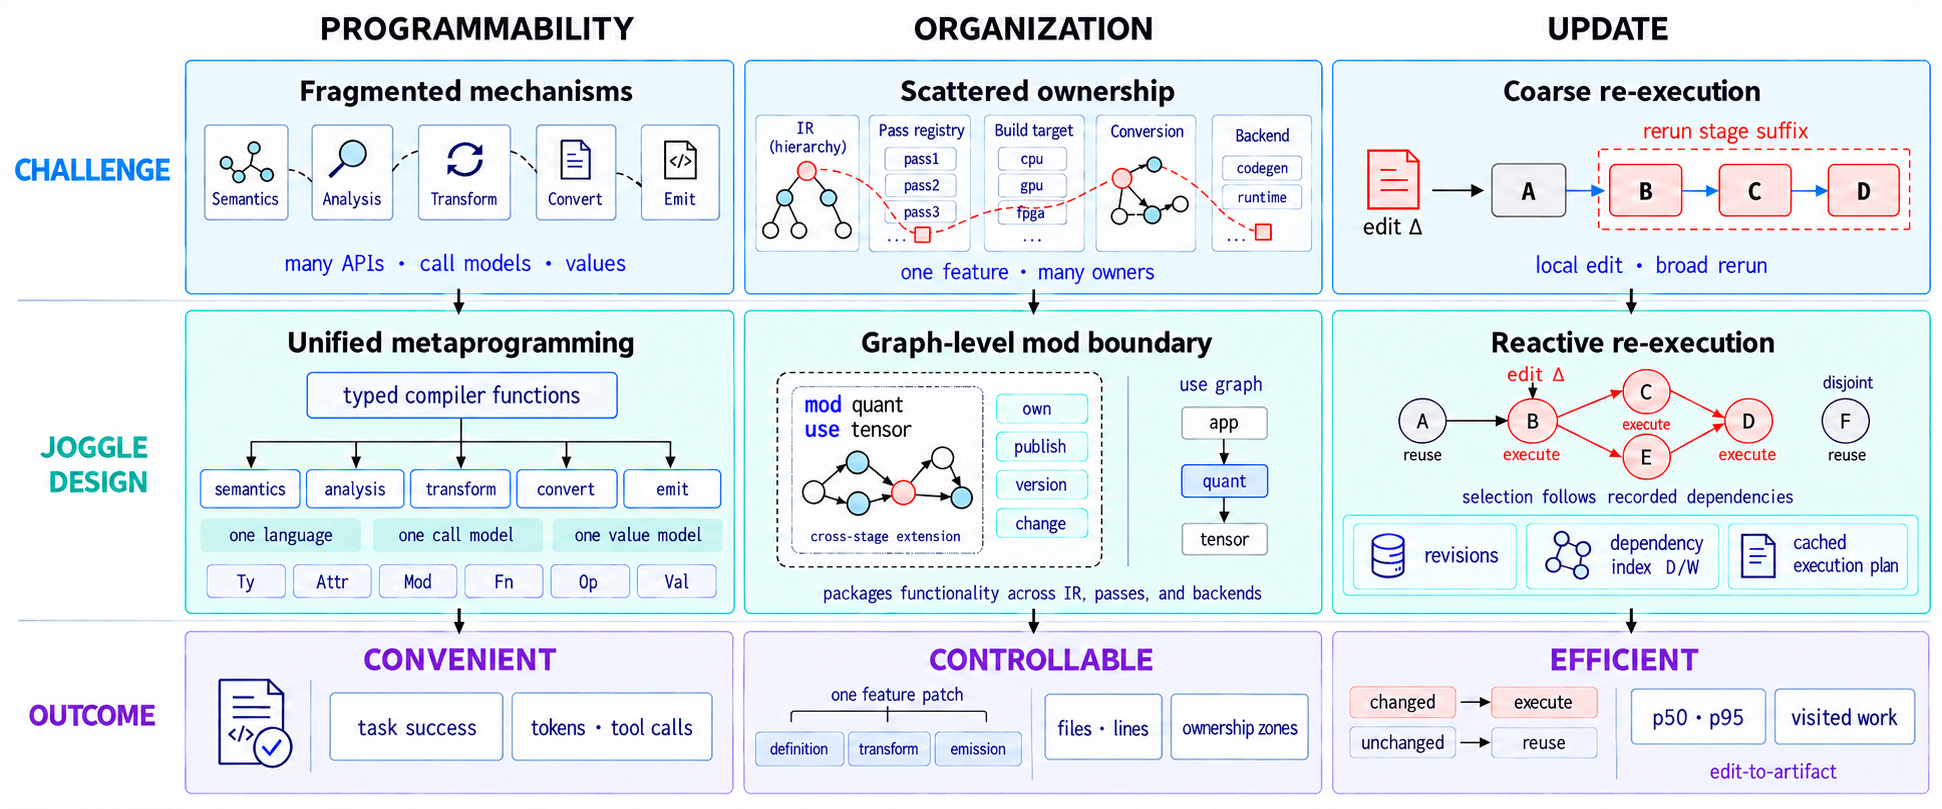
\includegraphics[width=.94\textwidth]{figures/figure-01-thesis-map.png}
  \caption{Joggle maps three extension challenges to system mechanisms and
    measurable outcomes.}
  \Description{A three-column, three-row argument map read top to bottom.
    Fragmented mechanisms map to unified metaprogramming and convenient
    extension. Scattered ownership maps to a graph-level mod boundary and
    controllable change. Coarse re-execution maps to revisions, dependency
    indices, cached plans, and efficient updates.}
  \label{fig:thesis-map}
\end{figure*}

Joggle addresses these problems by making compiler behavior part of the
program model. A Joggle program and its compiler extensions use the same typed
graph and the same function language. Analyses, transformations, converters,
and artifact generators are ordinary typed \emph{compiler functions}. A
\emph{mod} owns such functions with its graph, native bindings, and explicit
\texttt{use} dependencies. An evaluator executes calls transactionally,
observes the graph state they read, and records the effects they publish.

We call the representation \emph{progressive} because compilation proceeds
through typed refinements of one verified graph. A mod may retain semantic
operations, introduce lower-level
helpers, or replace selected definitions; each published intermediate remains
an inspectable Joggle mod. Progress is therefore chosen by typed functions and
explicit dependencies, not encoded as a mandatory global pipeline.

This design yields three contributions.

\paragraph{Unified metaprogramming.}
One language, call model, and value model cover semantic definitions, analyses,
graph transformations, representation conversion, and artifact generation
while retaining distinct read and write contracts.

\paragraph{Mod-scoped composition.}
Graph-level mod packages define ownership, publication, dependency, and change
boundaries across compilation stages. This boundary is orthogonal to
hierarchical program IR.

\paragraph{Dependency-directed updates.}
Revisions, dependency indices, and cached execution plans restrict
re-execution to compiler calls and stages whose recorded observations overlap
published edits, under transactional publication.

The evaluation assigns one evidence stream to each contribution. Held-out
extensions measure predictability and executable task success. Matched feature
patches measure repository footprint. Controlled edits over complete models
measure latency and executed work. Artifact quality and mechanism costs
complete the evidence chain while reporting compiler responsiveness and
generated-code quality separately.
